\section{Задание 4. Потенциал векторного поля}

\textbf{Условие.}

Дано векторное поле $\overrightarrow{H} = \left(\frac{1}{x^2}; \frac{1}{y^2}\right)$

Выполните:
\begin{enumerate}
    \item Убедитесь, что данное векторное поле потенциально.

    \item Найдите уравнения векторных линий. Изобразите векторные линии на рисунке.

    \item Найдите потенциал поля при помощи криволинейного интеграла.

    \item Найдите уравнения линий уровня потенциала (эквипотенциальных линий). Изобразите линии уровня потенциала.

    \item Докажите ортогональность найденных векторных линий поля и линий уровня потенциала. Проиллюстрируйте ортогональность на графике.

    \item Выберите какую-либо векторную линию поля и зафиксируйте на ней точки A и B, выбрав для них числовые координаты. Вычислите работу поля вдоль этой линии, используя найденный в п. 3) потенциал.


\end{enumerate}

\vspace{10mm}
\textbf{Решение.}

\begin{enumerate}
    \item Обозначим $\displaystyle P(x, y) = \frac{1}{x^2}, Q(x, y) = \frac{1}{y^2}, \overrightarrow{H} = (P, Q)$.

    Если поле потенциально, то вне зависимости от выбора пути \enquote{работа} от одной точки до другой должна быть равной.

    По теореме об интеграле, независящего от пути,
    поле называется потенциальным или безвихревым, если $\frac{\partial P}{\partial y} = \frac{\partial Q}{\partial x} \Longleftrightarrow \left(\frac{1}{x^2}\right)_y^\prime = \left(\frac{1}{y^2}\right)_x^\prime$, что выполняется, поэтому наше поле потенциальное

    Векторное поле выглядит так:

    \begin{center}
        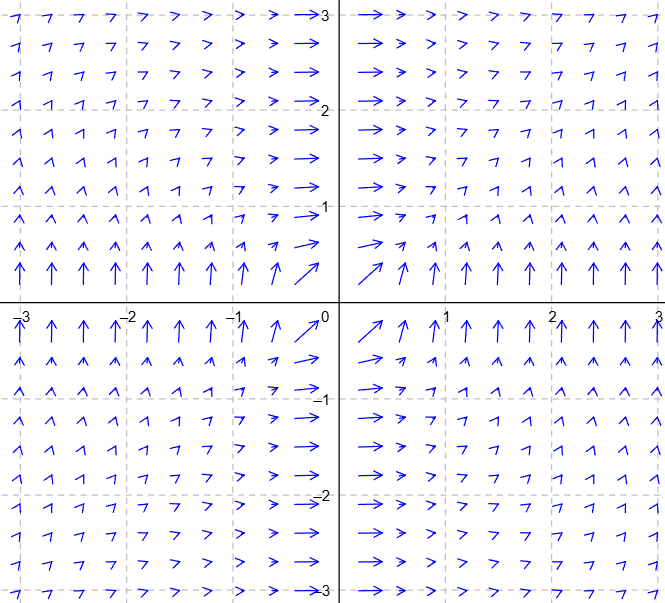
\includegraphics[height=80mm]{images/4a1}
    \end{center}

    \item По определению, векторные линии удовлетворяют уравнению $\frac{dx}{P} = \frac{dy}{Q} \Longleftrightarrow x^2 dx = y^2 dy \Longleftrightarrow y^3 = x^3 + C$

    Векторные линии при разных $C$ выглядят так:

    \begin{center}
        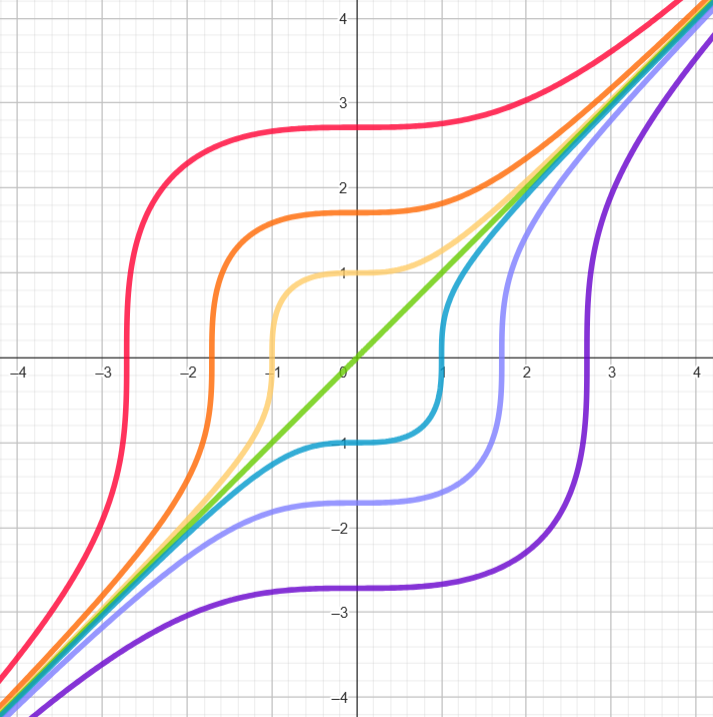
\includegraphics[height=80mm]{images/4b1}
    \end{center}

    \item Потенциалом поля называется такое поле $\overrightarrow{u}$, что $\overrightarrow{\triangledown}\overrightarrow{u} = \overrightarrow{H}$

    Тогда: $\frac{\partial u}{\partial x} = P, \frac{\partial u}{\partial y} = Q$

    $\displaystyle \begin{cases}\frac{\partial u}{\partial x} = \frac{1}{x^2}, \\ \frac{\partial u}{\partial y} = \frac{1}{y^2}\end{cases} \Longrightarrow
    \begin{cases}u = -\frac{1}{x} + f(y), \\ u = -\frac{1}{y} + g(x)\end{cases} \Longrightarrow u = -\frac{1}{x} - \frac{1}{y}$

    \item Линии уровня потенциала определяется по уравнению $u = -\frac{1}{x} - \frac{1}{y} = k$, где $k$ - потенциал на этой линии

    Тогда $\displaystyle y = -\frac{x}{1 + kx}$, график некоторых эквипотенциальных линий:

    \begin{center}
        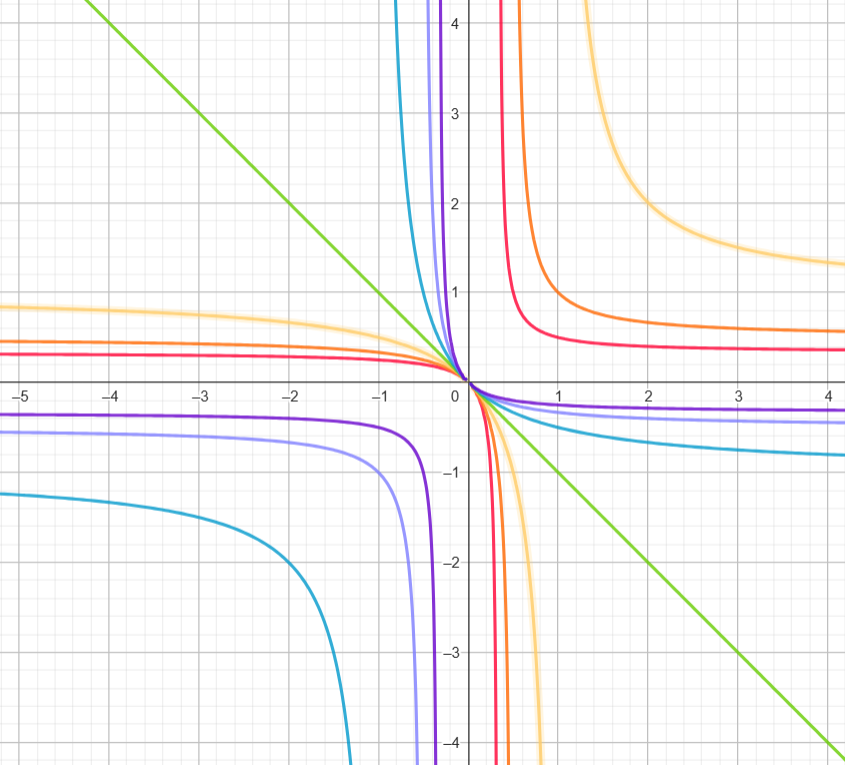
\includegraphics[height=80mm]{images/4d1}
    \end{center}


    \item Линии поля ортогональны, если они не пересекаются, значит $y^3 = x^3 + C_1$ и $y^3 = x^3 + C_2$ не имеют точек пересечения при различных $C_1$ и $C_2$

    $x^3 + C_1 = y^3 \neq y^3 = x^3 + C_2$

    $C_1 \neq C_2$ - тождество

    Аналогично для линии потенциалов:

    $\displaystyle -\frac{x}{1 + C_1 x} \neq -\frac{x}{1 + C_2 x} \quad x \neq 0$ - поле неопределенно при $x = 0$

    $1 + C_1 x \neq 1 + C_2 x$

    $C_1 \neq C_2$ - тождество

    \item Пусть у векторной линии коэффициент $C = 3$, тогда выберем такие $A$ и $B$, что $y^3 = x^3 + 8$, пусть $A = (1, \sqrt[3]{9})$, $B = \left(4, 2\sqrt[3]{9}\right)$

    Тогда $\displaystyle \int_A^B Pdx + Qdy = u(B) - u(A) = -\frac{1}{x_B} - \frac{1}{y_B} + \frac{1}{x_A} + \frac{1}{y_A} =
    -\frac{1}{4} - \frac{1}{2\sqrt[3]{9}} + \frac{1}{1} + \frac{1}{\sqrt[3]{9}} =
    \frac{3}{4} + \frac{1}{2\sqrt[3]{9}} = \frac{3}{4} + \frac{\sqrt[3]{81}}{18}$

    \begin{center}
        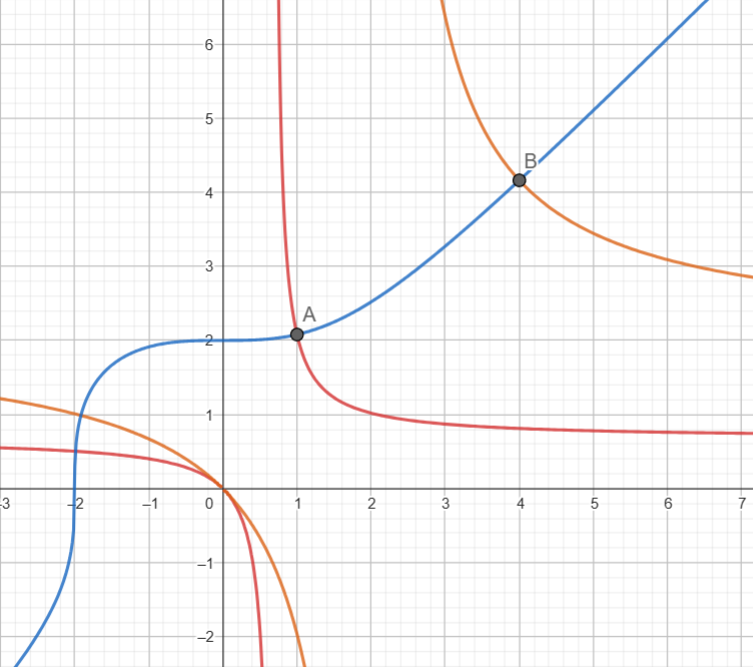
\includegraphics[height=80mm]{images/4e1}
    \end{center}

    Проверим: $\displaystyle \int_A^B Pdx + Qdy = \int_{(1, \sqrt[3]{9})}^{(4, \sqrt[3]{9})} Pdx + Qdy + \int_{(4, \sqrt[3]{9})}^{(4, 2\sqrt[3]{9})} Pdx + Qdy =
    \int_{(1, \sqrt[3]{9})}^{(4, \sqrt[3]{9})} \frac{1}{x^2}dx + \int_{(4, \sqrt[3]{9})}^{(4, 2\sqrt[3]{9})} \frac{1}{y^2}dy =
    -\frac{1}{x} \Big|_{(1, \sqrt[3]{9})}^{(4, \sqrt[3]{9})} - \frac{1}{y} \Big|_{(4, \sqrt[3]{9})}^{(4, 2\sqrt[3]{9})} =
    -\frac{1}{4} + \frac{1}{1} + (-\frac{1}{2\sqrt[3]{9}} + \frac{1}{\sqrt[3]{9}}) =
    \frac{3}{4} + \frac{1}{2\sqrt[3]{9}}$ - верно


\end{enumerate}

\clearpage
